\chapter[Attitude Estimation with CV]{Attitude Estimation with Computer Vision}
\thispagestyle{empty}
\section{Vision Hardware and Experimental Setup}
\begin{table}[h]
    \centering
    \begin{tabular}{|c|c|c|c|}
        \hline
        \textbf{Component} & \textbf{Model/Version} & \textbf{Role} & \textbf{Cost} \\
        \hline
        Raspberry Pi 5 & 8GB RAM & Frame acquisition and attitude computation & 85€ \\
        \hline
        Right Pi Camera & V3 & Capture right frame & 27€ \\
        \hline
        Left Pi Camera & V3 & Capture left frame & 27€ \\
        \hline
        Heatsink & Active & CPU cooling & 11€ \\
        \hline
        SanDisk Extreme & 64GB & OS storage & 15€ \\
        \hline
        \textbf{Total} & & & \textbf{165€} \\
        \hline
    \end{tabular}
    \caption{Components used for attitude estimation}
    \label{tab:example}
\end{table}

The computer vision part consists of a pair of rigidly mounted and calibrated cameras. The baseline is 12 cm, also measured during calibration. The cameras operate at a resolution of 1280$\times$720 px with a frame rate of 30 fps, providing an excellent compromise between visual quality and required resources.

The calibration procedure is performed live by framing the calibration checkerboard. Calibrations are carried out for each camera (focal length, principal point, and distortion) and subsequently for the stereo pair (rotation and translation). At the end of the calibration, the files are saved and later loaded by the attitude estimation program.

The visual reference for estimation is a single \textbf{ArUco marker} (in our case, a 6$\times$6 dictionary) with a known size. The marker is printed on a rigid and opaque support to reduce potential problems caused by reflections. The marker size must be such that it remains visible even at a distance, since the acquisition resolution is limited.

Each cycle for the estimation calculation begins with the rectification of the cameras using the previously acquired calibration files. Subsequently, if the marker is detected, the algorithm proceeds to the next step. If present, the four vertices are triangulated to reconstruct the 3D coordinates. The reconstructed points are compared with the theoretical model of the marker, thus allowing the estimation of the \textbf{complete pose} (rotation and translation) using the \textit{estimateAffine3D} method. The rotation is converted to quaternions to avoid 180° jumps in the measurements. Finally, the video stream is displayed with the real-time attitude estimation, showing roll, pitch, and yaw on the screen.

The measurement quality is ensured by checking, in each frame, that all marker corners are visible for correct identification. In this case, the combination of stereo vision, ArUco marker, and pose estimation using the \textit{estimateAffine3D} method provides stable and reliable attitude estimates.

\section{Stereo Camera Calibration}

\begin{figure}[ht]
  \centering
  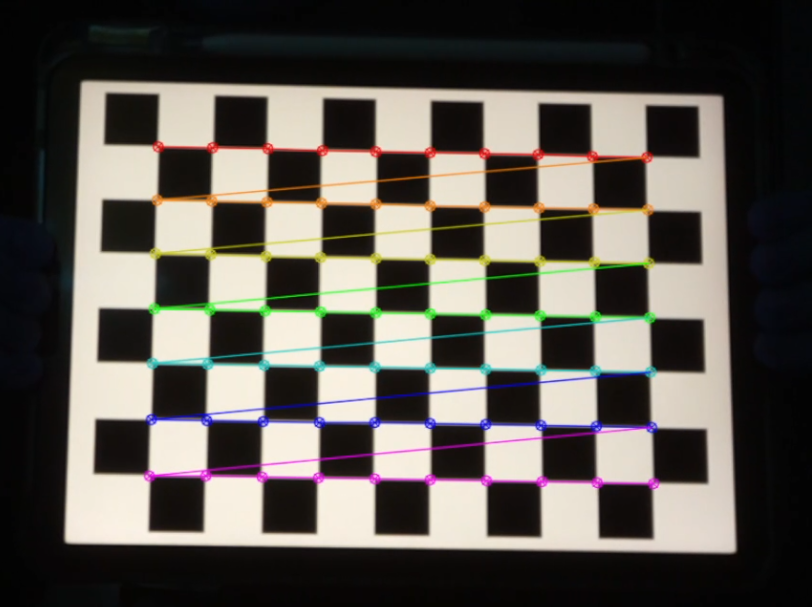
\includegraphics[height=6cm]{images/calib.png}
  \caption{Checkerboard pattern with detected feature points during camera calibration.}
\end{figure}

The calibration of the \textbf{stereo cameras} was implemented through an algorithm that performs a \textit{live acquisition} of a checkerboard of known size, used as a reference. The two cameras are rigidly mounted on a \textbf{bracket} to avoid movements and acquire the images of the calibration pattern. For each acquired frame, the inner corners of the checkerboard are detected in both frames, subsequently the coordinates are made more accurate through \textbf{sub-pixel precision}. This procedure is repeated for each acquisition frame (in our case 50 frames), in order to collect a sufficiently high number of samples to make our calibration more \textit{stable}.

Once the acquisition of the frames is completed, the calibration of the \textbf{individual cameras} is performed. For each camera, the fundamental optical parameters are calculated, represented by: focal length, principal point and lens distortion. These parameters are essential to correct the radial and tangential distortions created by the optics, thus ensuring a faithful representation of \textbf{reality}.

The next part is \textbf{stereo calibration}, which allows estimating the geometric relationship between the two cameras. Thanks to the common points of the pattern, the algorithm calculates the rotation matrix and the translation vector of the right camera with respect to the left one. To ensure consistency with the physical setup, the translation vector is scaled so that the \textbf{baseline} is exactly 12 cm, that is the real distance between the two cameras.

Finally, the matrices necessary to realign the images and ensure the subsequent triangulation of the points in space are calculated. All the parameters are saved in different files, so that they can be used by the program that estimates the \textit{attitude}.

\section{Detection of ArUco markers}

Detection of ArUco markers is fundamental for our \textbf{computer vision pipeline}, as it represents a reliable visual reference to be used in the subsequent phases of attitude estimation. ArUco markers are black squares containing a unique binary pattern, \textit{easily distinguishable} even under difficult lighting conditions. They are designed to minimize ambiguities that may occur between different markers, ensuring stable and fast recognition.
\\Each frame acquired by the cameras is processed by the function\\ \texttt{detectMarkers}, which is responsible for detecting the markers present within the frames. The algorithm uses a 6x6 marker dictionary. Once detected, both the coordinates of the vertices and the marker ID are returned; all this information will be used in the subsequent parts of the algorithm.
\\To improve the accuracy of the algorithm, the OpenCV library provides the \texttt{DetectorParameters} structure, which allows adjusting some detection parameters. In our case, we exclusively use \texttt{CORNER\_REFINE\_SUBPIX}, which allows achieving \textbf{sub-pixel precision} in the detection of the vertices. This is particularly useful when the marker is observed at long distances.
\\An important aspect concerns candidate markers that are subsequently discarded. During frame analysis, there may be regions that resemble the searched marker but do not contain a valid code. These are discarded but can still be visualized and analyzed through the function \texttt{refineDetectedMarkers}, which is especially useful when aiming to develop a particularly stable and robust system.
\\In conclusion, the detection process provides a \textbf{fast and reliable response} in identifying the markers present in the scene, returning the necessary information such as their ID and vertex positions. These data, once validated, are the essential starting point for the subsequent phases of triangulation and attitude estimation, thus ensuring \textit{consistency and reliability} throughout the process.

\section{Pose Estimation Algorithms}

The estimation of the boat’s attitude represents the \textbf{most important phase} of the entire pipeline, as it precisely determines the position of the boat with respect to the marker in three-dimensional space, in reference to the stereo camera system.  

The process begins with the detection of the marker in the two rectified frames. In both frames, the markers are identified and subsequently the vertices corresponding to the corners of the square are extracted. These points, once extracted, are used to perform triangulation through the \textit{triangulatePoints} function, which reconstructs the 3D coordinates of the vertices in a common space. The result is a set of 3D points in space that describe the geometry of the marker.
In parallel, an \textbf{ideal marker model} is defined in the reference system. This model has known dimensions, specified in the program (in our case 12 cm), whose vertices are described in the plane \(z = 0\). The goal is to find the rigid transformation that maps the ideal model to coincide with the 3D points previously reconstructed. 

To obtain the transformation, we use the \textit{estimateAffine3D} function, which returns an affine matrix \(A\), consisting of the rotation matrix \(R\) and the translation vector \(T\). The rotation describes the orientation of the marker, while the translation its position with respect to the stereo system.  

The rotation matrix is then converted into quaternions using the \textbf{SciPy} library, in order to eliminate the ambiguities of the Euler angles. The quaternions are subsequently transformed into Euler angles (\textit{roll}, \textit{pitch}, and \textit{yaw}) for a quicker interpretation.  

Finally, to guarantee the \textbf{temporal continuity} of the estimation and avoid sign changes, a consistency check between the current pose and the pose of the previous frame has been implemented.  

The implemented algorithm, as described, makes it possible to obtain a \textbf{robust and fast estimation} with respect to a marker, thus providing a basis for the kinematic models of the system.

\begin{figure}[ht]
  \centering
  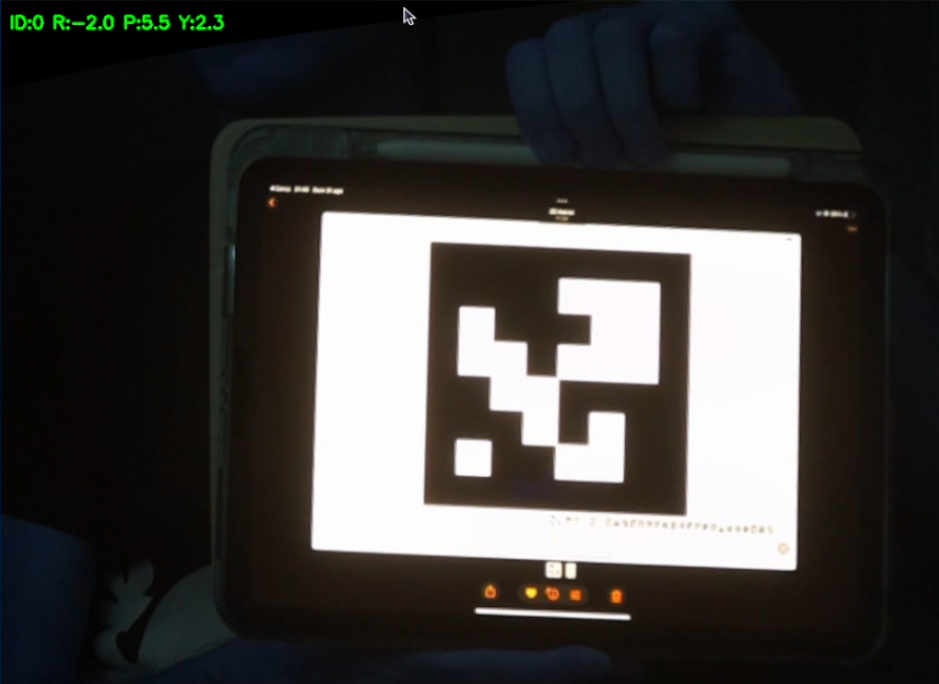
\includegraphics[height=6cm]{images/roll_pitch_yaw.png}
  \caption{Detection of an ArUco marker with estimated roll, pitch, and yaw values displayed.}
\end{figure}

\section[Limitations and Critical Issues]{Limitations and Critical Issues of the Visual Method}

The stereo camera approach to the problem of attitude estimation, using \textbf{ArUco markers}, offers several advantages in terms of \textit{simplicity}, cost, and ease of implementation. Nevertheless, there are several \textbf{limitations and challenges} that must be taken into account to ensure reliable use in a marine scenario.

The first aspect to consider concerns the dependence on \textbf{lighting conditions}. The accuracy with which the marker is detected may deteriorate in the presence of strong light, pronounced shadows, or reflections. Although ArUco markers are designed to provide stable recognition, certain conditions may lead to \textit{false negatives} or errors in the detection of corners.

The second aspect to be considered is the \textbf{distance and angle of observation}. If the marker is observed from a great distance or with a considerable tilt, the edges appear less defined and the detection function may return points that are not very accurate. This results in a deterioration of triangulation and the subsequent pose estimation, especially regarding the accuracy of quaternions and thus the calculation of Euler angles.

Another critical aspect concerns \textbf{stereo triangulation}. For the algorithm to work, it relies on the correspondence of points in the two rectified frames. If the frames are misaligned due to calibration issues or uncompensated distortion, the three-dimensional reconstruction may be inaccurate, negatively affecting the transformation estimated by the function \texttt{estimateAffine3D}.

The issue of \textbf{false positives} must also be considered. In certain conditions, visual patterns may resemble a marker and therefore be mistakenly identified as such. Although functions like \texttt{refineDetectedMarkers} help to mitigate the problem, in complex systems this risk cannot be entirely eliminated.

The last critical aspect is \textbf{temporal continuity}. Although controls are in place to avoid sign flips in the quaternions, if tracking is lost or interruptions occur in the marker detection, discontinuities in the estimation may arise, leading to oscillations in roll, pitch, and yaw values.

In summary, the method based on ArUco markers and stereo vision provides an efficient and low-cost solution, but it presents limitations due to \textit{environmental conditions} and the sensitivity of the cameras. For an application like ours, these limitations must be considered and, if necessary, compensated by additional sensors that complement the estimation.
